\chapter{A Numerical Evaluation of the PEM} \label{ch:results}
%
\section{Convergence Analysis}

\subsection*{Infinite Elastic Plate in Far-Field Tension}

\begin{figure}[!h]
  \centering
  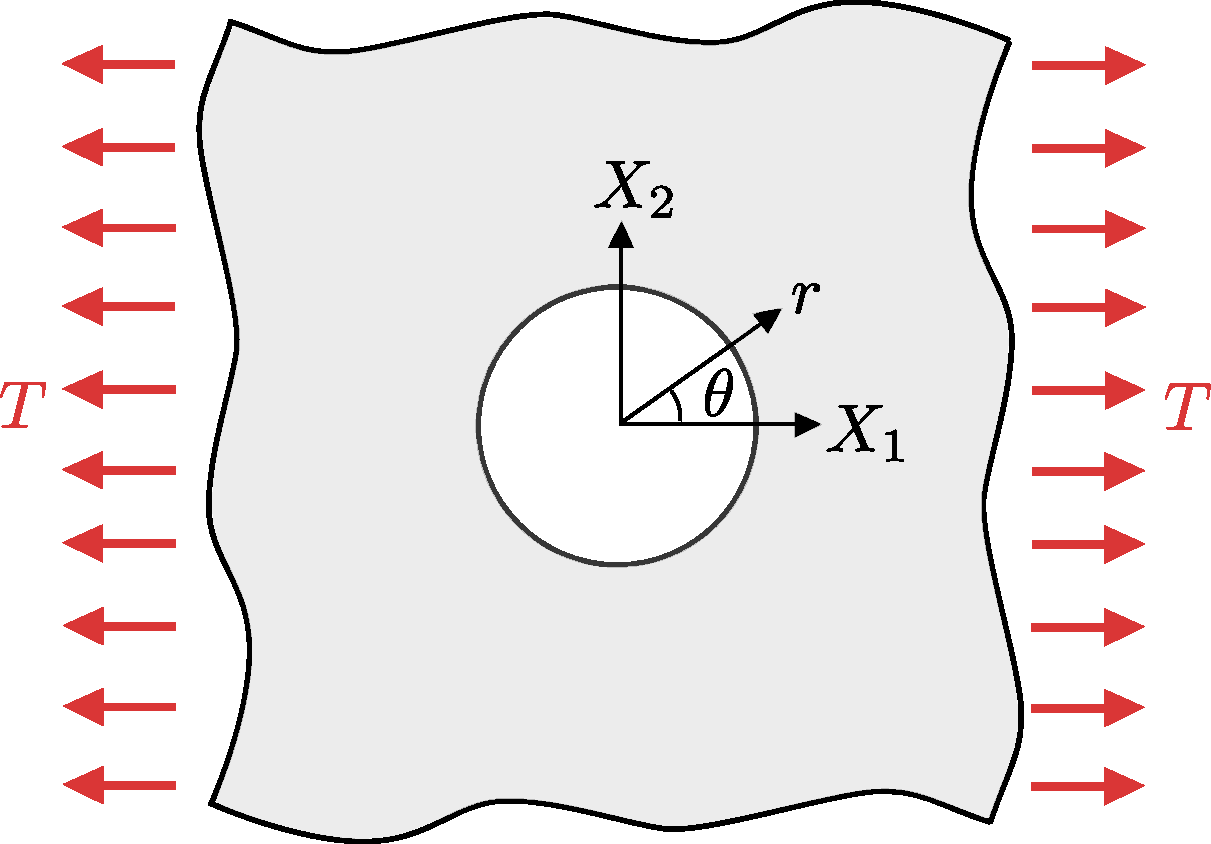
\includegraphics[width=4.0in]{figures/plate_with_hole.pdf}  \caption{Infinite plate with a circular hole placed in uniaxial tension.}
  \label{fig:plate_with_hole_problem}
\end{figure}
To demonstrate optimal convergence of the PEM for higher-order elements, we will choose to investigate the 2D elastostatics problem of an infinite plate with a circular hole in uniaxial tension (depicted in figure \ref{fig:plate_with_hole_problem}), for which there exist analytical solutions of the resulting displacement and stress fields (obtained from reference \cite{Wikiversity:17}):
\begin{equation}
  u_1 (r,\theta) = \frac{Ta}{8\mu} \left[ \frac{r}{a} (\kappa + 1) \cos \theta + \frac{2a}{r} ((1+\kappa) \cos \theta + \cos 3 \theta) - \frac{2a^3}{r^3} \cos 3 \theta \right]
\end{equation}
\begin{equation}
  u_2 (r,\theta) = \frac{Ta}{8\mu} \left[ \frac{r}{a} (\kappa - 3) \sin \theta + \frac{2a}{r} ((1-\kappa) \sin \theta + \sin 3 \theta) - \frac{2a^3}{r^3} \sin 3 \theta \right]
\end{equation}
\begin{equation}
  \sigma_{11} (r, \theta) = T - T \frac{a^2}{r^2} \bigg( \frac{3}{2} \cos 2 \theta + \cos 4 \theta \bigg) + T \frac{3a^4}{2r^4} \cos 4 \theta
\end{equation}
\begin{equation}
  \sigma_{22} (r, \theta) = - T \frac{a^2}{r^2} \bigg( \frac{1}{2} \cos 2 \theta - \cos 4 \theta \bigg) - T \frac{3a^4}{2r^4} \cos 4 \theta
\end{equation}
\begin{equation}
  \sigma_{12} (r, \theta) = - T \frac{a^2}{r^2} \bigg( \frac{1}{2} \sin 2 \theta + \sin 4 \theta \bigg) + T \frac{3a^4}{2r^4} \sin 4 \theta
\end{equation}
where $T$ is the far-field value of the applied tensile stress, $a$ is the radius of the circular hole centered at $r=0$, $\kappa = 4 - 3\nu$ (under plane-strain conditions), and $\nu$ and $\mu$ are the the Poisson's ratio and shear modulus of the material, respectively.

\begin{figure}[!h]
  \centering
  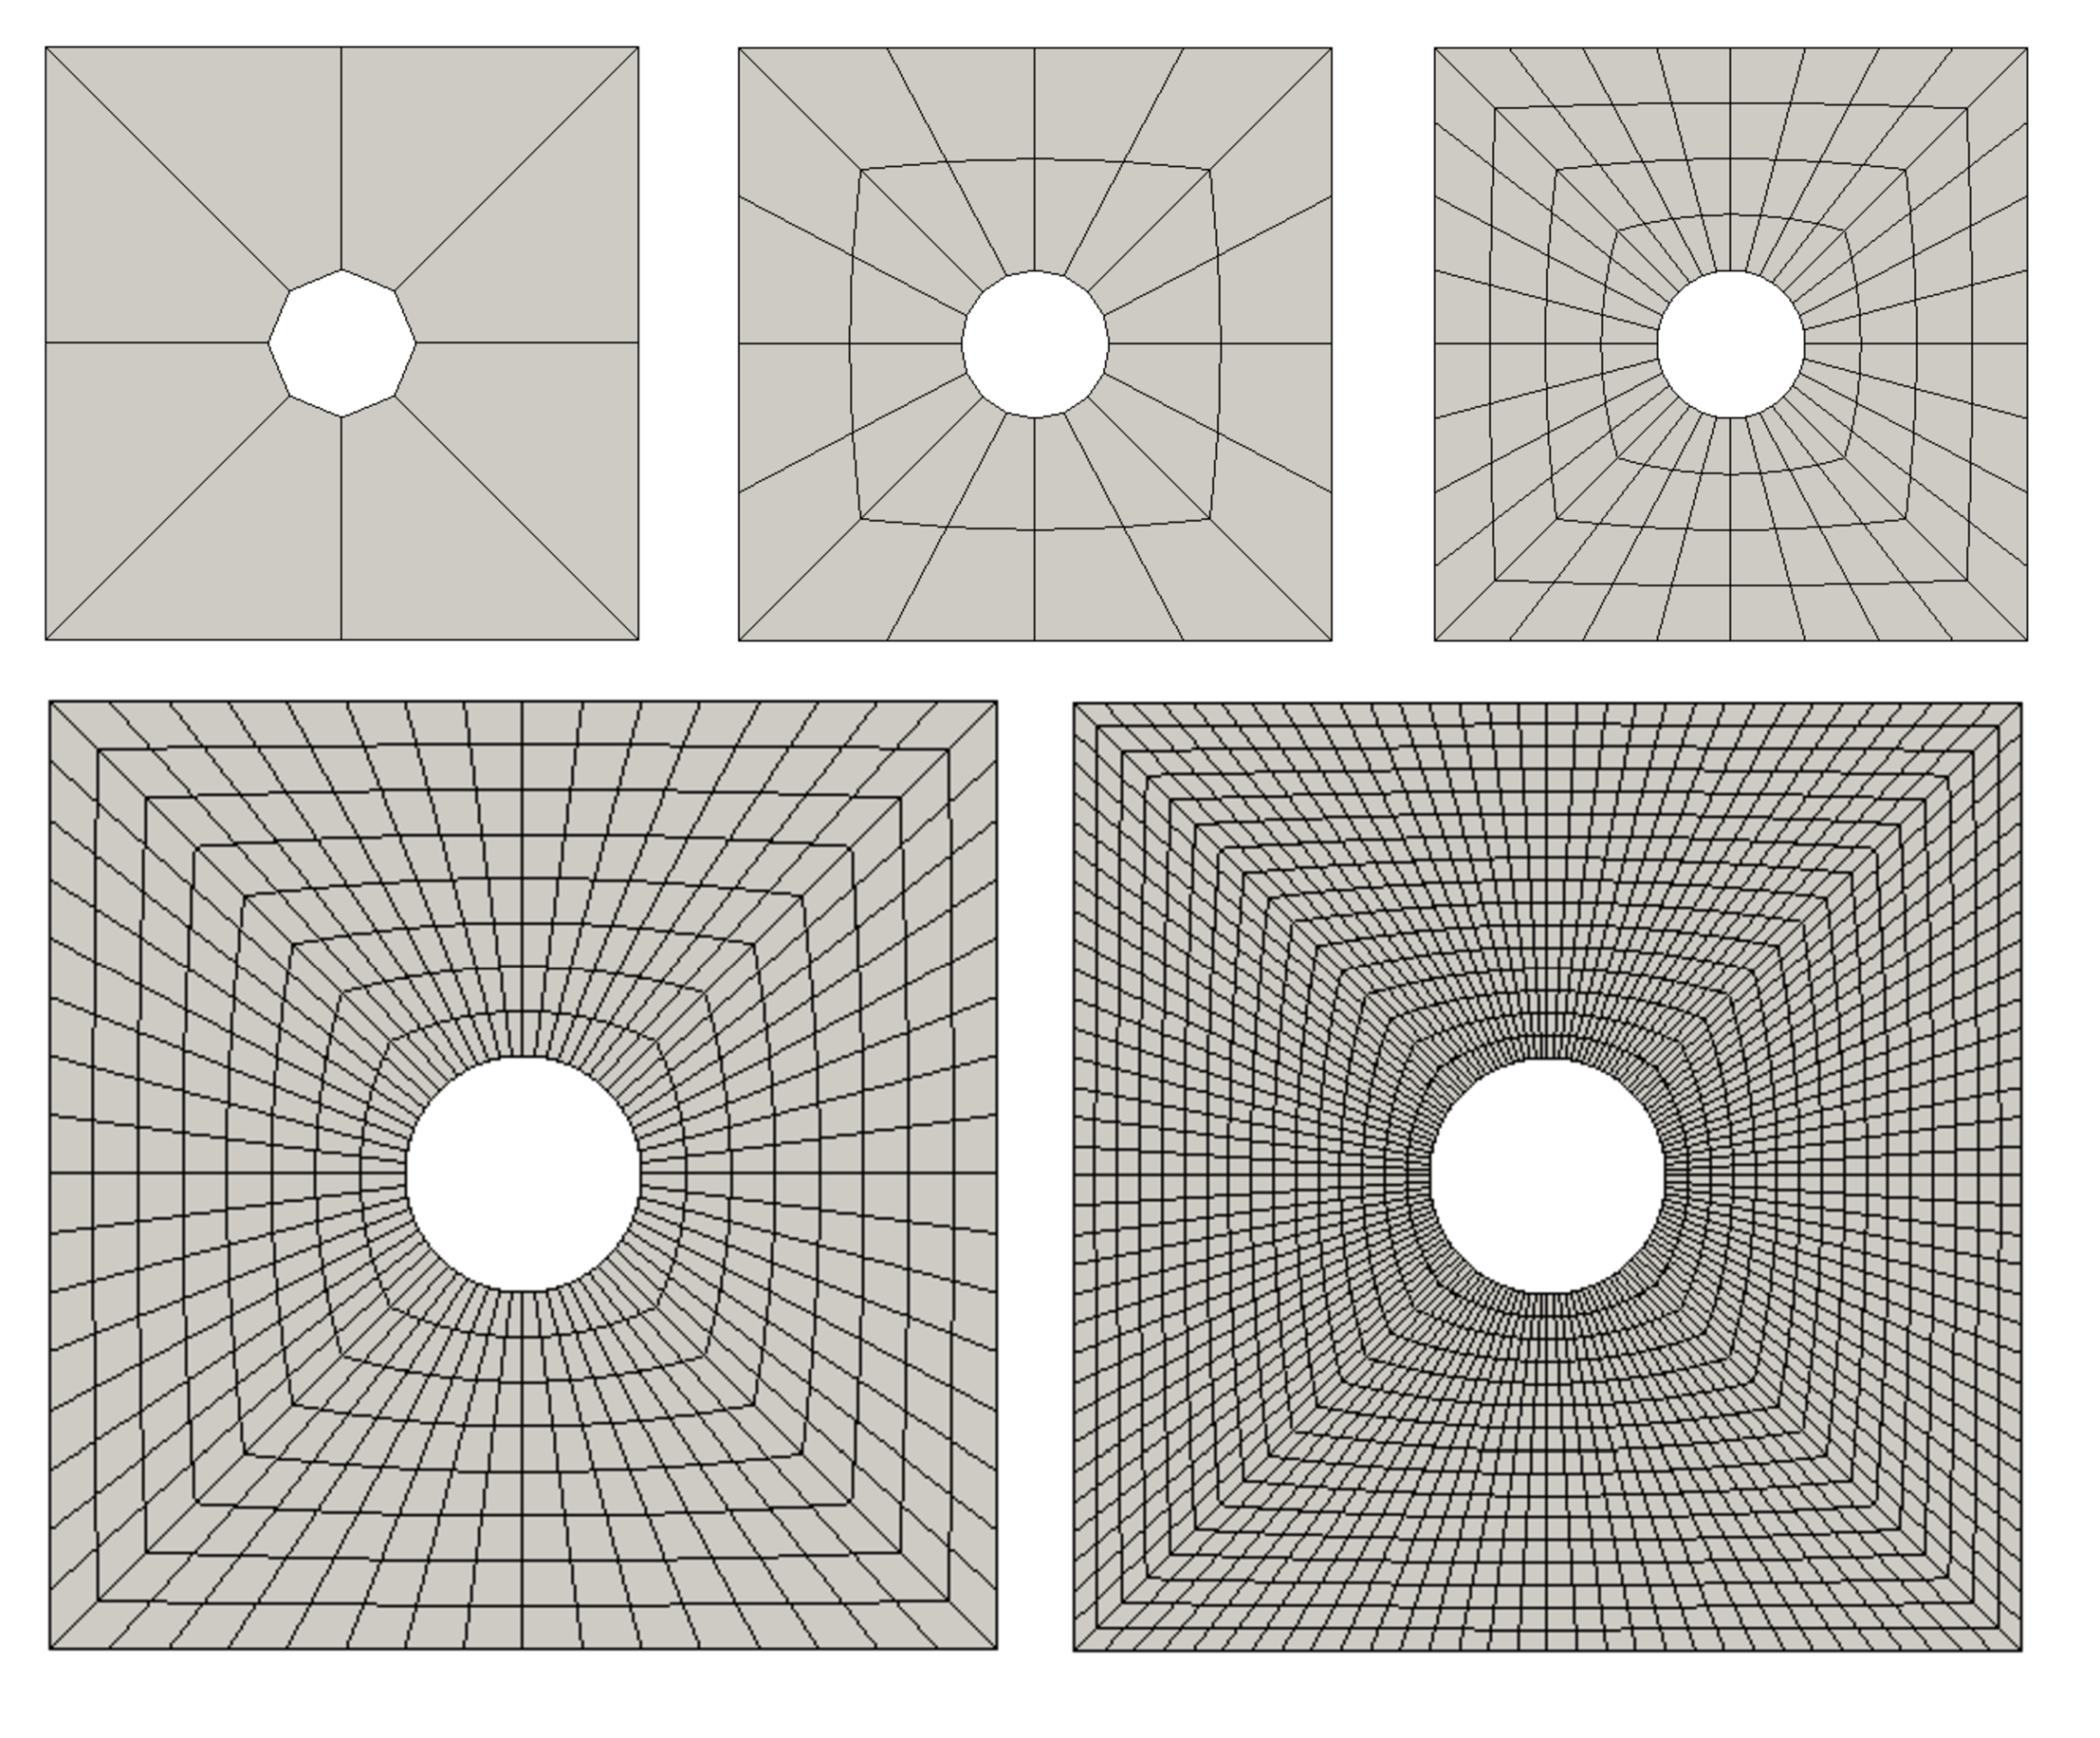
\includegraphics[width=6.0in]{figures/plate_with_hole_meshes.pdf}
  \caption{Quadrilateral meshes with varying levels of refinement.}
  \label{fig:plate_with_hole_meshes}
\end{figure}
A convergence study was carried out using a series of quadrilateral meshes with varying levels of refinement discretizing the restricted problem domain $X_i \in [ -1, +1]$ (see figure \ref{fig:plate_with_hole_meshes}.) The meshes consisted of either 4-node quadrilateral or 8-node serendipity quadrilateral elements, and employed either an isoparametric formulation, or a sufficiently high-order PEM formulation (i.e. $k=1$ for 4-node quadrilaterals, and $k=2$ for 8-node quadrilaterals.) Displacement boundary conditions were prescribed to be consistent with the exact solution on the restricted boundary. $L^2$ displacement error norms and $H^1$ energy error semi-norms were computed with reference to the exact solution, with the numerical results summarized in tables \ref{tab:l2_error}-\ref{tab:h1_rates}. The convergence rates in the $L^2$ and $H^1$ error norms are depicted in figures \ref{fig:l2_error} and \ref{fig:h1_error}, respectively.
\newpage
\begin{table}[!ht]
  \begin{center}
    \begin{tabular}{| c | c | c | c | c |}
    \hline
    $h$ & 4-node FEM & 4-node PEM & 8-node FEM & 8-node PEM \\ \hline
    1.2500 & 1.3133E-006 & 1.4901E-006 & 9.8369E-007 & 2.9990E-006 \\ \hline
    0.8006 & 6.9557E-007 & 9.8453E-007 & 4.8165E-007 & 1.3918E-006 \\ \hline
    0.4488 & 2.8755E-007 & 4.2859E-007 & 2.2034E-007 & 3.3673E-007 \\ \hline
    0.2371 & 1.0460E-007 & 1.3672E-007 & 8.1971E-008 & 4.8942E-008 \\ \hline
    0.1218 & 3.1430E-008 & 3.7296E-008 & 2.4628E-008 & 6.7201E-009 \\ \hline
    0.0617 & 8.3877E-009 & 9.5661E-009 & 6.5479E-009 & 1.6002E-009 \\
    \hline
    \end{tabular}
    \caption{Computed $L^2$ displacement error norms.}
    \vspace{-5pt}
    \label{tab:l2_error}
    \vspace{-25pt}
  \end{center}
\end{table}
\begin{table}[!ht]
  \begin{center}
    \begin{tabular}{| c | c | c | c | c |}
    \hline
    $h$ & 4-node FEM & 4-node PEM & 8-node FEM & 8-node PEM \\ \hline
    1.2500 &	-	&	-	&	-	&       -      \\ \hline
    0.8006 &	1.4265	&	0.9302	&	1.6028	&	1.7230 \\ \hline
    0.4488 &	1.5262	&	1.4369	&	1.3512	&	2.4518 \\ \hline
    0.2371 &	1.5848	&	1.7906	&	1.5496	&	3.0225 \\ \hline
    0.1218 &	1.8051	&	1.9502	&	1.8053	&	2.9808 \\ \hline
    0.0617 &	1.9424	&	2.0007	&	1.9479	&	2.1100 \\
    \hline
    \end{tabular}
    \caption{Computed $L^2$ displacement error norm convergence rates.}
    \vspace{-5pt}
    \label{tab:l2_rates}
    \vspace{-25pt}
  \end{center}
\end{table}
\begin{table}[!ht]
  \begin{center}
    \begin{tabular}{| c | c | c | c | c |}
    \hline
    $h$ & 4-node FEM & 4-node PEM & 8-node FEM & 8-node PEM \\ \hline
    1.2500 & 2.1468E-001 & 2.8913E-001 & 1.8275E-001 & 5.3700E-001 \\ \hline
    0.8006 & 1.8622E-001 & 2.5620E-001 & 1.5959E-001 & 3.0529E-001 \\ \hline
    0.4488 & 1.3786E-001 & 1.7930E-001 & 1.2495E-001 & 1.5310E-001 \\ \hline
    0.2371 & 9.2075E-002 & 1.1251E-001 & 7.9144E-002 & 5.8671E-002 \\ \hline
    0.1218 & 5.2124E-002 & 6.2223E-002 & 4.2868E-002 & 1.5541E-002 \\ \hline
    0.0617 & 2.7048E-002 & 3.2135E-002 & 2.1789E-002 & 3.3672E-003 \\
    \hline
    \end{tabular}
    \caption{Computed $H^1$ energy error semi-norms.}
    \vspace{-5pt}
    \label{tab:h1_error}
    \vspace{-25pt}
  \end{center}
\end{table}
\begin{table}[!ht]
  \begin{center}
    \begin{tabular}{| c | c | c | c | c |}
    \hline
    $h$ & 4-node FEM & 4-node PEM & 8-node FEM & 8-node PEM \\ \hline
    1.2500 &	-	&	-	&	-	&       -      \\ \hline
    0.8006 &	0.3192	&	0.2714	&	0.3042	&	1.2675 \\ \hline
    0.4488 &	0.5195	&	0.6166	&	0.4228	&	1.1924 \\ \hline
    0.2371 &	0.6326	&	0.7303	&	0.7156	&	1.5031 \\ \hline
    0.1218 &	0.8542	&	0.8892	&	0.9205	&	1.9944 \\ \hline
    0.0617 &	0.9646	&	0.9716	&	0.9950	&	2.2488 \\
    \hline
    \end{tabular}
    \caption{Computed $H^1$ energy error semi-norm convergence rates.}
    \vspace{-5pt}
    \label{tab:h1_rates}
    \vspace{-25pt}
  \end{center}
\end{table}
\begin{figure}[!h]
  \centering
  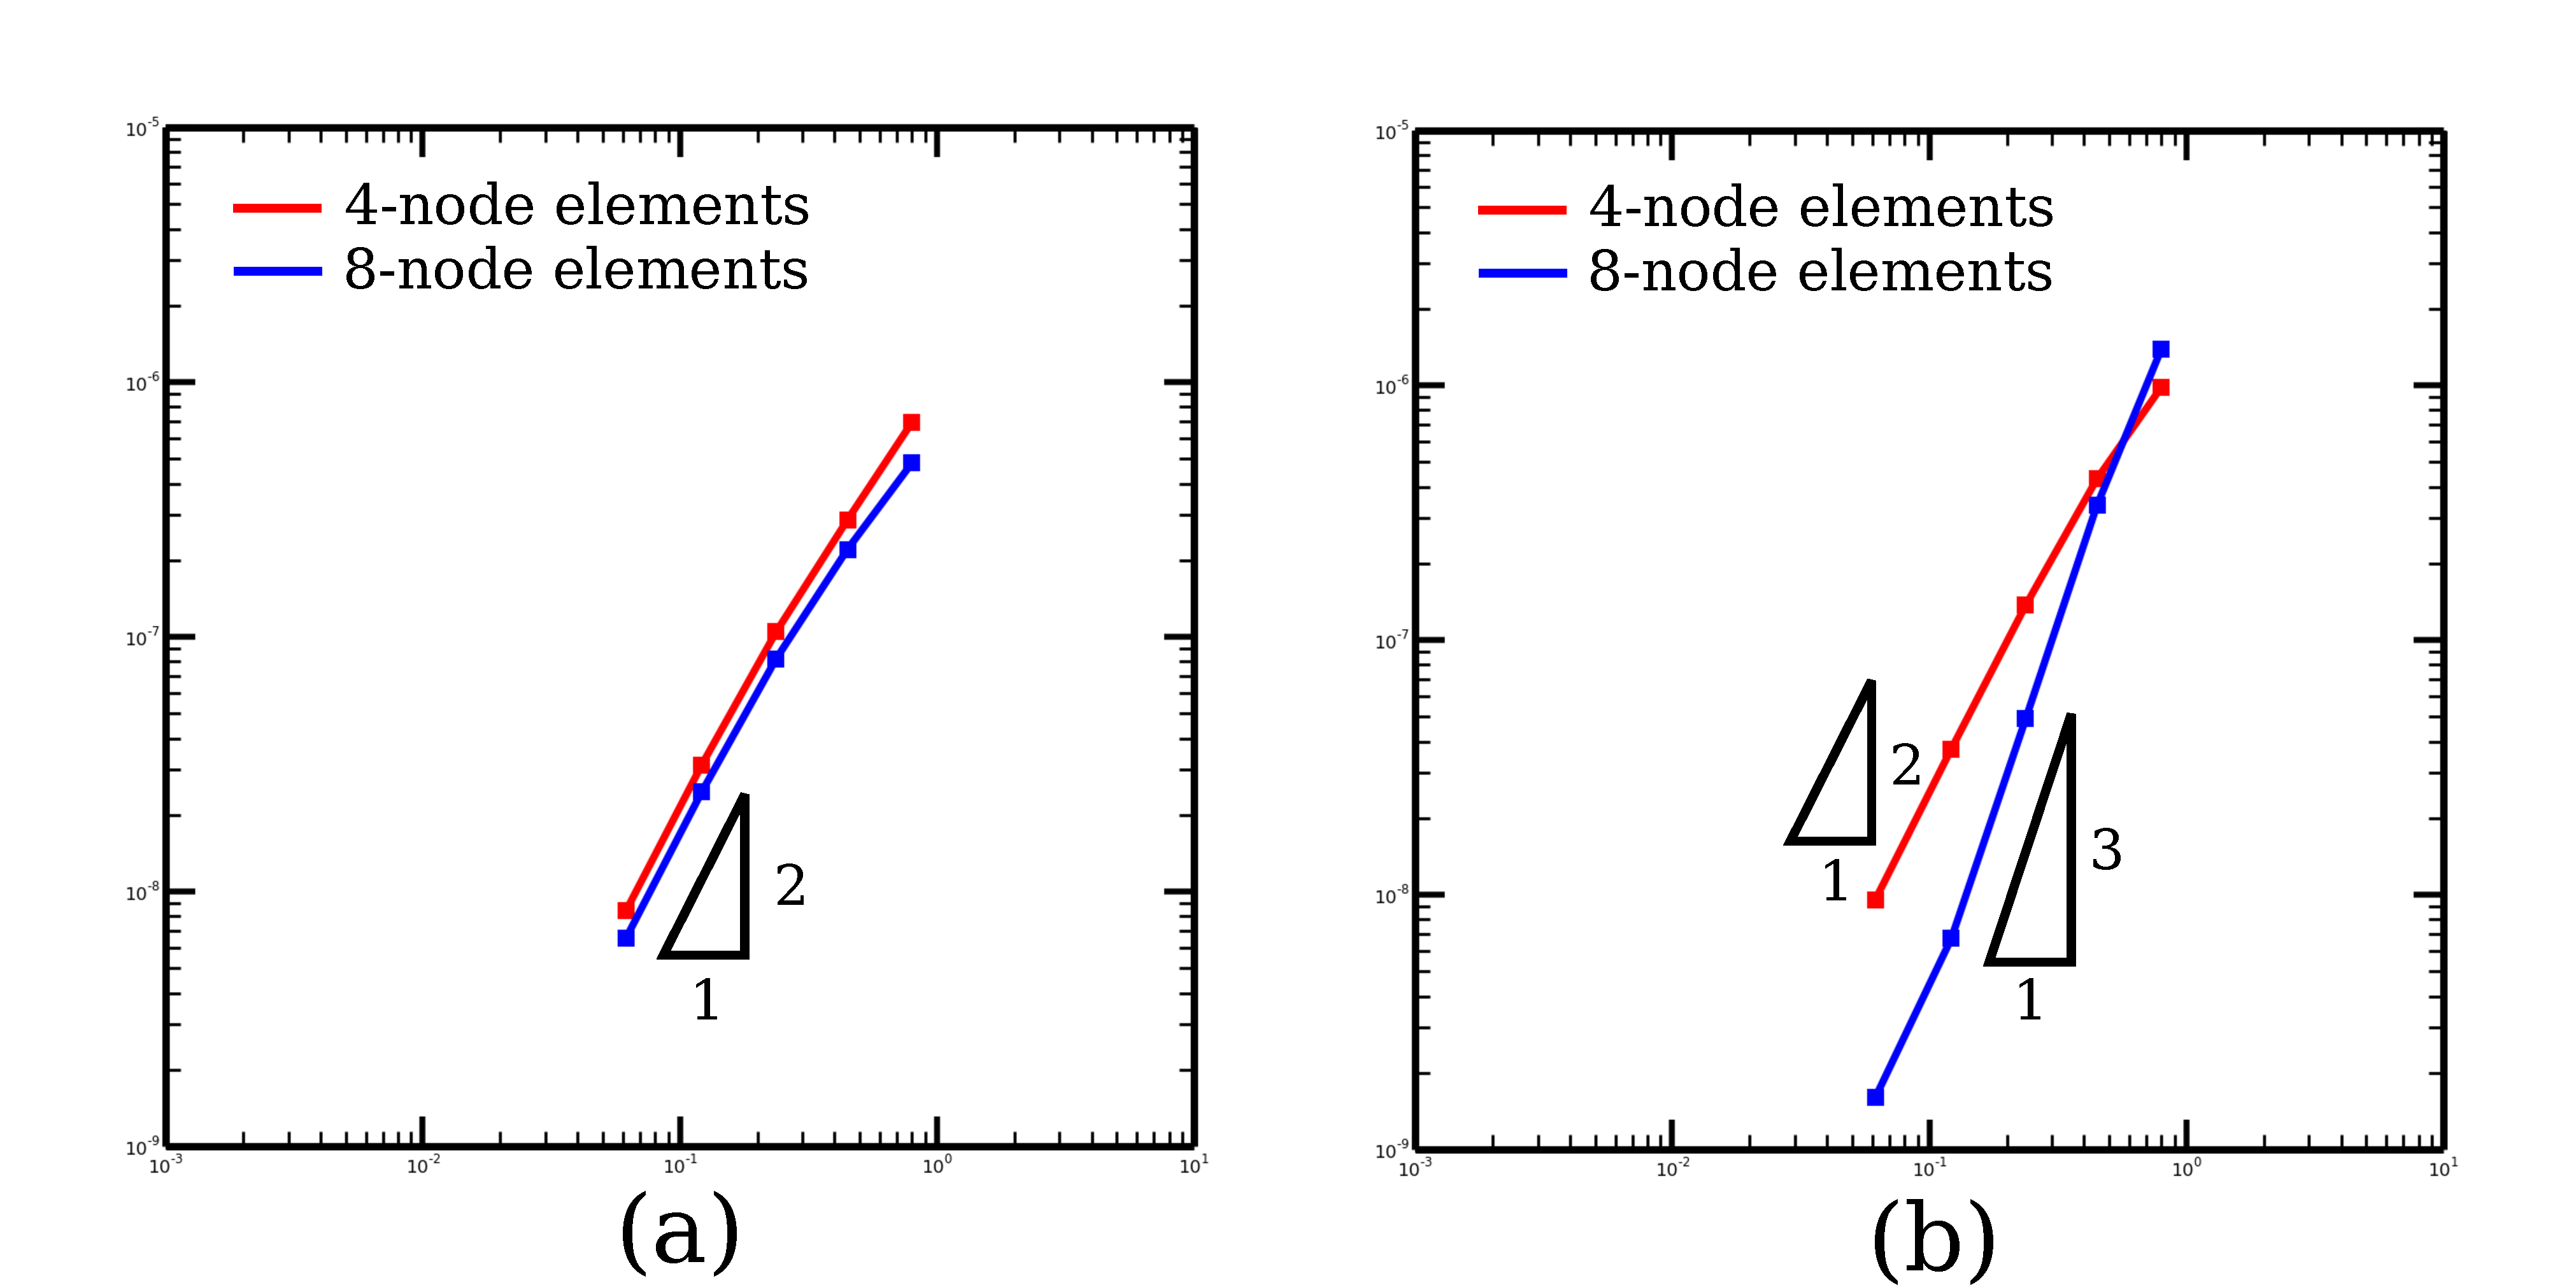
\includegraphics[width=6.0in]{figures/l2_error_plot.pdf}
  \caption{$L^2$ error convergence plots for (a) FEM and (b) PEM formulations.}
  \label{fig:l2_error}
  \vspace{-10pt}
\end{figure}

\begin{figure}[!h]
  \centering
  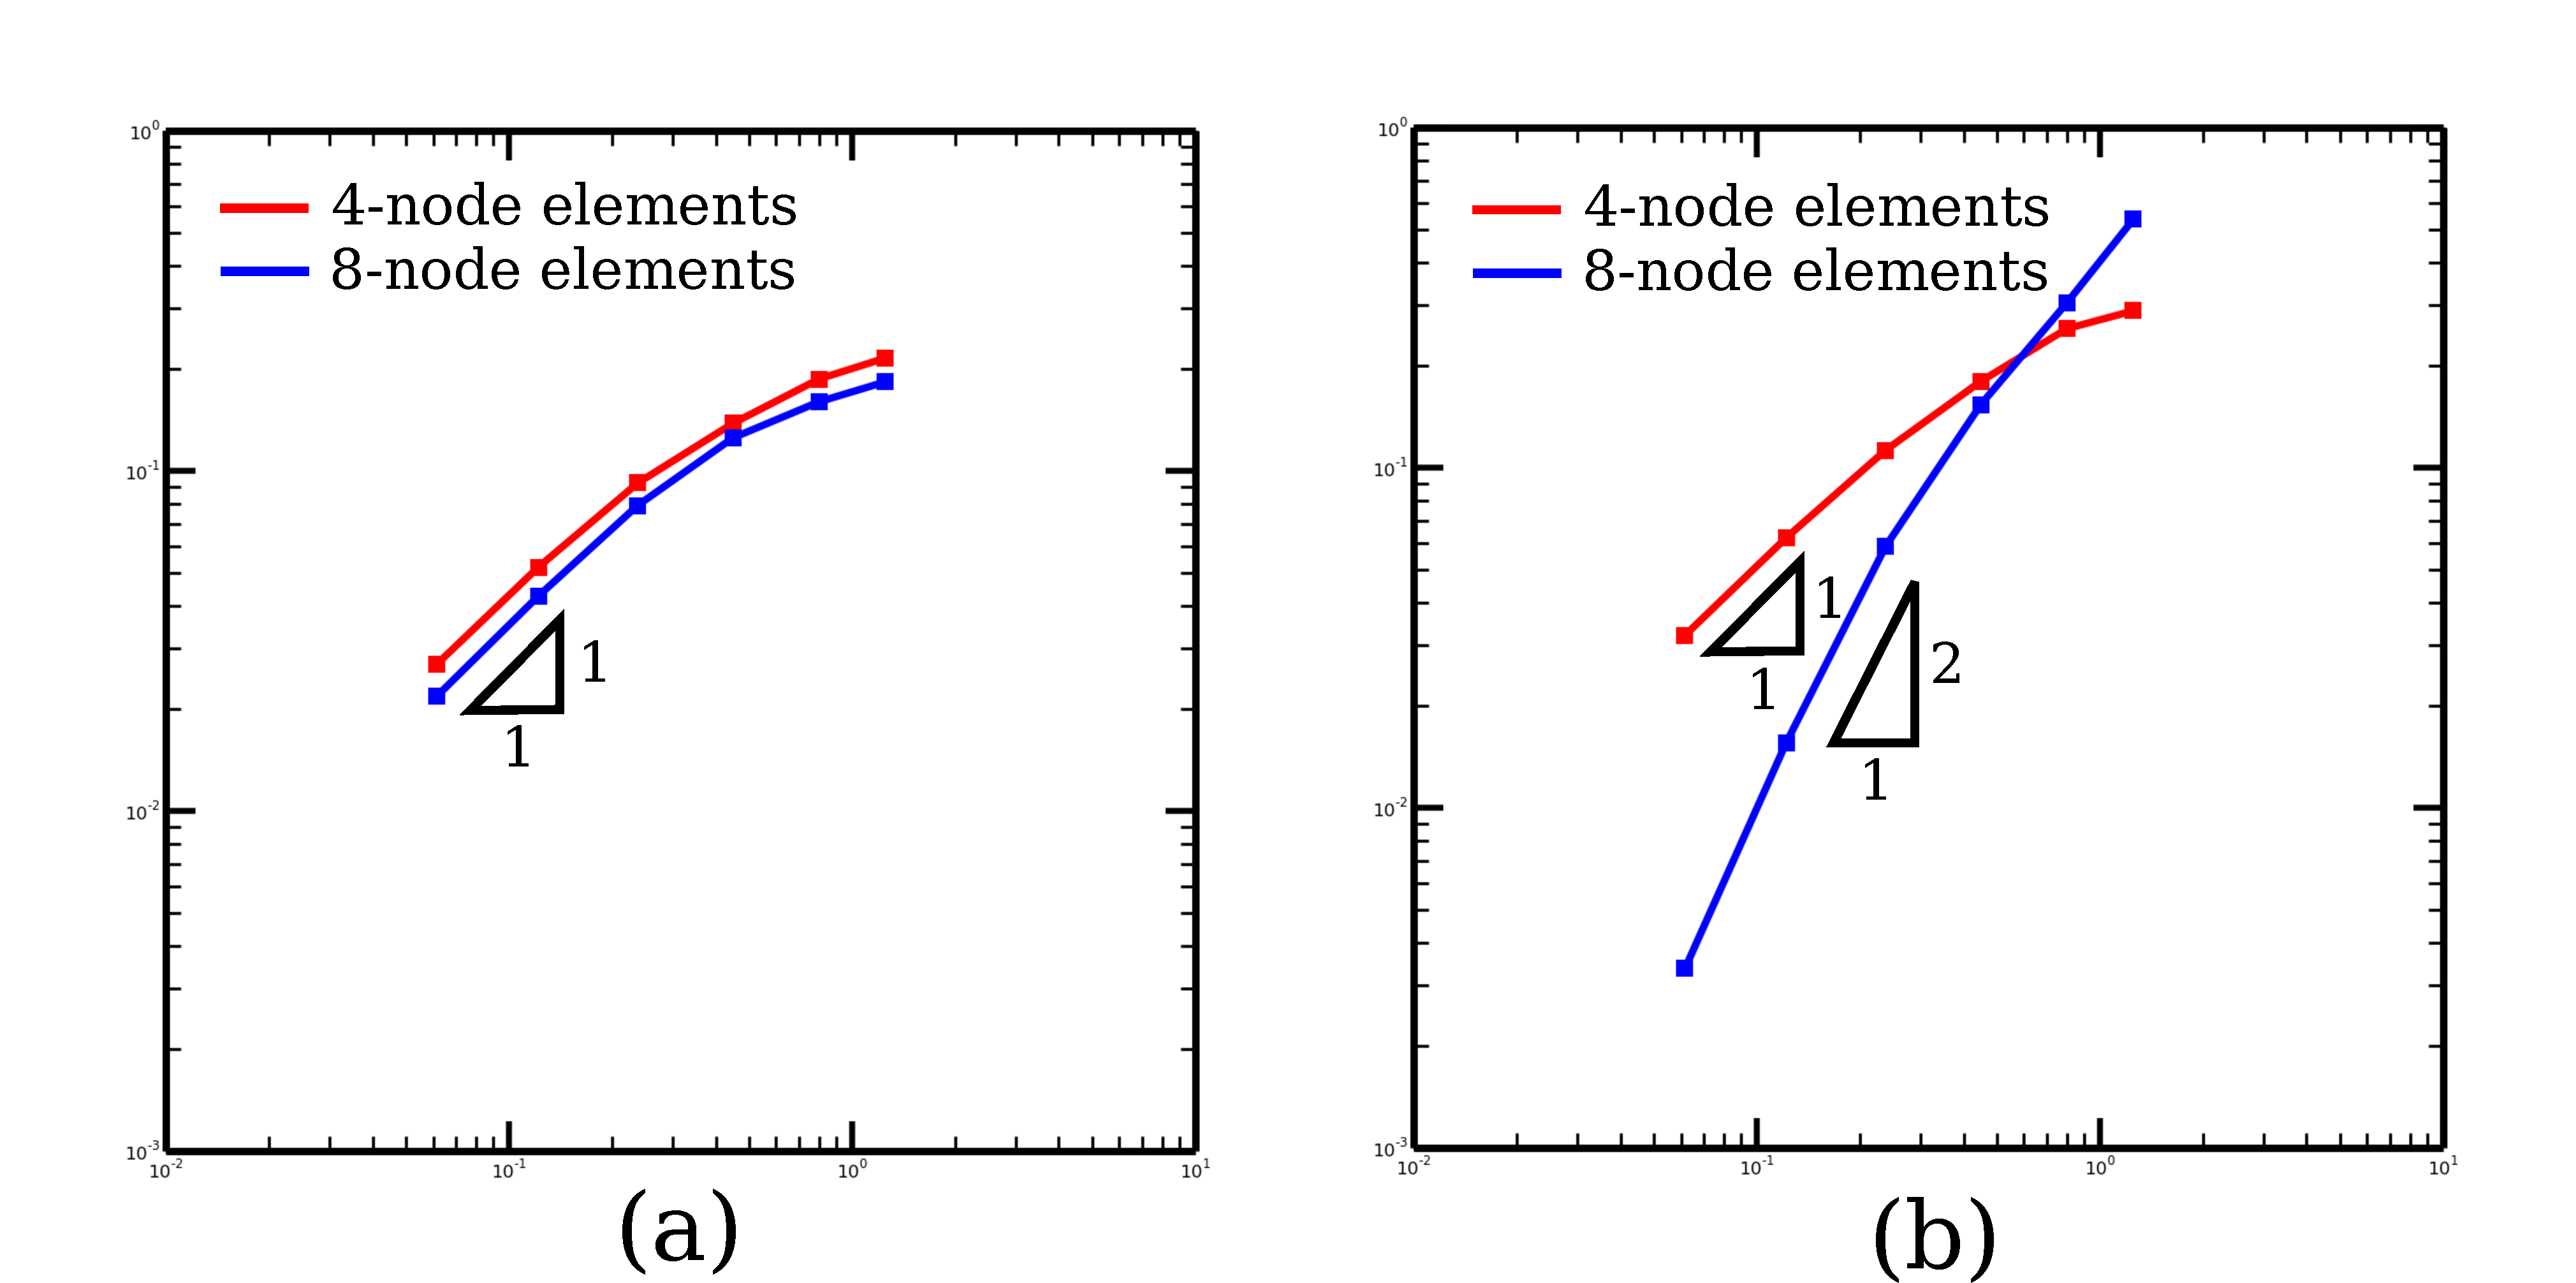
\includegraphics[width=6.0in]{figures/h1_error_plot.pdf}
  \caption{$H^1$ error convergence plots for (a) FEM and (b) PEM formulations.}
  \label{fig:h1_error}
\end{figure}

A number of observations should be made regarding the resulting data. In particular, it is worthwhile to note that part of the incurred solution error may be attributable to the inexact representation of the problem geometry, especially for the coarse meshes. This may in part explain why the observed convergence rates are lower at coarser levels of refinement, but approach the expected rates as the mesh is further refined.

Additionally, we remark that isoparametric serendipity quadrilateral elements converge at sub-optimal rates if the elements are distorted in a non-affine fashion (as is the case for our meshes). This is an altogether expected result, and has been discussed in references \cite{Arnold:01} and \cite{Arnold:02}.

Conversely, we observe that the PEM quadrilateral elements converge at the optimal rates in both the $L^2$ and $H^1$ error norms, as we would hope.

Further work will seek to investigate the measured error and convergence rates of the PEM when the elements take on arbitrary shape, and for a variety of different formulations and penalization parameter settings.

\section{Parameter Sensitivity Analysis}

\section{Computational Efficiency}
\subsection{Performance Comparison}

\section{Resistance to Locking Phenomena}

\subsection*{Twisting Annulus}

Consider an incompressible elastic annulus whose inner radius at $r = R_i$ is fixed, and whose outer radius $r = R_o$ rigidly rotates at an angular velocity of $\Phi$. The radially symmetric displacement boundary conditions for this motion are described by
\begin{equation}
	u_r (R_i,t) = u_r (R_o,t) = 0, \quad u_z (R_i,t) = u_z (R_o,t) = 0,
\end{equation}
\begin{equation}
	u_\theta (R_i,t) = 0, \quad u_\theta (R_o,t) = R_o \, \Phi \, t,
\end{equation}
for all $t \geq 0$.

The elastic material is characterized by a linear hypoelastic material model of grade zero, obeying
\begin{equation}
  \dot{\boldsymbol{\sigma}} = \mathbb{C} : \mathbf{D} + \mathbf{W} \boldsymbol{\sigma} - \boldsymbol{\sigma} \mathbf{W},
\end{equation}

\subsubsection*{Exact Solution}

An exact solution for the aforementioned problem may be obtained by considering the stress divergence equations in cylindrical polar coordinates:
\begin{equation}
  \nabla \cdot \boldsymbol{\sigma} = \left\{ \begin{array}{c} \frac{\partial \sigma_{rr}}{\partial r} + \frac{\sigma_{rr}}{r} + \frac{1}{r} \frac{\partial \sigma_{\theta r}}{\partial \theta} + \frac{\partial \sigma_{z r}}{\partial z} - \frac{\sigma_{\theta \theta}}{r} \\
    \frac{1}{r} \frac{\partial \sigma_{\theta \theta}}{\partial \theta} + \frac{\partial \sigma_{r\theta}}{\partial r} + \frac{\sigma_{r\theta}}{r} + \frac{\sigma_{\theta r}}{r} + \frac{\partial \sigma_{z \theta}}{\partial z} \\
    \frac{\partial \sigma_{z z}}{\partial z} + \frac{\partial \sigma_{r z}}{\partial r} + \frac{\sigma_{r z}}{r} + \frac{1}{r} \frac{\partial \sigma_{\theta z}}{\partial \theta} \end{array} \right\} = \mathbf{0}.
\end{equation}
By the assumptions of plane strain and axisymmetry, we rationalize that $\boldsymbol{\sigma} (r)$ is a function of $r$, alone, and therefore,
\begin{equation}
  \nabla \cdot \boldsymbol{\sigma} = \left\{ \begin{array}{c} \frac{\partial \sigma_{rr}}{\partial r} + \frac{\sigma_{rr} - \sigma_{\theta \theta}}{r} \\
    \frac{\partial \sigma_{r\theta}}{\partial r} + \frac{2 \sigma_{r\theta}}{r} \\
    \frac{\partial \sigma_{r z}}{\partial r} + \frac{\sigma_{r z}}{r} \end{array} \right\} = \mathbf{0}.
\end{equation}
Furthermore, by the assumptions of plane strain, we observe that $\sigma_{rz} = 0$ and $\sigma_{\theta z} = 0$. Additionally, if we impose the incompressibility condition $\nabla \cdot \mathbf{v} = \text{tr} (\mathbf{D}) = 0$, we find that
\begin{equation}
  \text{tr} (\dot{\boldsymbol{\sigma}}) = 0 \, \Rightarrow \, \text{tr} (\boldsymbol{\sigma}) = 0 \, \forall t.
\end{equation}
The deformation necessitates that $\sigma_{zz} = 0$, and therefore $\sigma_{\theta \theta} = - \sigma_{rr}$. Consequently, we are left with 2 governing differential equations for $\sigma_{rr}$ and $\sigma_{r \theta}$:
\begin{equation}
  \frac{\partial \sigma_{rr}}{\partial r} + \frac{2 \sigma_{rr}}{r} = 0, \quad \frac{\partial \sigma_{r\theta}}{\partial r} + \frac{2 \sigma_{r\theta}}{r} = 0,
\end{equation}
whose solutions are of the form
\begin{equation}
  \sigma_{rr} = \frac{a}{r^2}, \quad \sigma_{r\theta} = \frac{b}{r^2}.
\end{equation}
Consequently,
\begin{equation}
  \left\{ \begin{array}{c} \sigma_{rr} \\ \sigma_{\theta \theta} \\ \sigma_{r \theta} \end{array} \right\} = r^{-2} \left\{ \begin{array}{c} +a \\ -a \\ b \end{array} \right\}.
\end{equation}

Under the assumption of incompressibility, we may characterize the deformation via the velocity field $v_r = 0$, $v_z = 0$, and $v_\theta (r) = r \dot{\phi}(r)$, yielding the velocity gradient (in cylindrical polar coordinates):
\begin{equation}
  \mathbf{L} = \nabla \mathbf{v} = \left[ \begin{array}{ccc} v_{r,r} & v_{r,\theta}/r-v_\theta /r & v_{r,z} \\
      v_{\theta,r} & v_{\theta,\theta}/r + v_r /r & v_{\theta,z} \\
      v_{z,r} & v_{z,\theta} /r & v_{z,z} \end{array} \right] = 
  \left[ \begin{array}{ccc} 0 & -\dot{\phi} & 0 \\
      \dot{\phi} + r \dot{\phi}_{,r} & 0 & 0 \\
      0 & 0 & 0 \end{array} \right],
\end{equation}
and the corresponding rate of deformation and spin tensors:
\begin{equation}
  \mathbf{D} = \frac{r \dot{\phi}_{,r}}{2} \left[ \begin{array}{ccc} 0 & 1 & 0 \\
      1 & 0 & 0 \\
      0 & 0 & 0 \end{array} \right], \quad \mathbf{W} = 
  \frac{2 \dot{\phi} + r \dot{\phi}_{,r}}{2} \left[ \begin{array}{ccc} 0 & - 1 & 0 \\
      1 & 0 & 0 \\
      0 & 0 & 0 \end{array} \right].
\end{equation}
The resulting stress rate equations are
\begin{equation}
  \left\{ \begin{array}{c} \dot{\sigma}_{rr} \\ \dot{\sigma}_{\theta \theta} \\ \dot{\sigma}_{r \theta} \end{array} \right\} = \left\{ \begin{array}{c} 0 \\ 0 \\ \mu r \dot{\phi}_{,r} \end{array} \right\} + 
  (2 \dot{\phi} + r \dot{\phi}_{,r}) \left\{ \begin{array}{c} - \sigma_{r \theta} \\ \sigma_{r \theta} \\ \sigma_{rr} \end{array} \right\},
\end{equation}
or
\begin{equation}
  \left\{ \begin{array}{c} \dot{a} \\ \dot{b} \end{array} \right\} = \left\{ \begin{array}{c} 0 \\ \mu r^3 \dot{\phi}_{,r} \end{array} \right\} + (2 \dot{\phi} + r \dot{\phi}_{,r}) \left[ \begin{array}{cc} 0 & -1 \\ 1 & 0 \end{array} \right] \left\{ \begin{array}{c} a \\ b \end{array} \right\},
\end{equation}
which must be valid $\forall r, \, t$. If we assume that $\dot{\phi} = f(r)$ is a function of $r$ (and not of $t$), then we obtain the condition
\begin{equation}
  3 f_{,r} + r f_{,rr} = 0,
\end{equation}
implying $f_{,r} = B r^{-3}$, and $\phi (r, t) = (A - B r^{-2} / 2)t$, thus
\begin{equation}
  \left\{ \begin{array}{c} \dot{a} \\ \dot{b} \end{array} \right\} = \left\{ \begin{array}{c} 0 \\ \mu B \end{array} \right\} + 2 A \left[ \begin{array}{cc} 0 & -1 \\ 1 & 0 \end{array} \right] \left\{ \begin{array}{c} a \\ b \end{array} \right\},
\end{equation}
and
\begin{equation}
  a(t) = - \frac{\mu B}{2 A} - C_2 \sin (2 A t) + C_1 \cos (2 A t),
\end{equation}
\begin{equation}
  b(t) = C_1 \sin (2 A t) + C_2 \cos (2 A t).
\end{equation}
Imposing the initial conditions $a(0) = b(0) = 0$ results in:
\begin{equation}
  a(t) = \frac{\mu B}{2 A} \left[ \cos (2 A t) - 1 \right], \quad b(t) = \frac{\mu B}{2 A} \sin (2 A t).
\end{equation}
Imposing the boundary conditions $\phi(R_i,t) = 0 \, \, \forall t$, $\phi(R_o,t) = \Phi \, t \, \, \forall t$ yields:
\begin{equation}
  A = \frac{\Phi R_i^{-2}}{R_i^{-2} - R_o^{-2}}, \quad B = \frac{2 \Phi}{R_i^{-2} - R_o^{-2}}.
\end{equation}

The final analytical solution for the displacement and stress fields is presented below:
\begin{equation}
  u_r = 0, \quad u_\theta = r \Phi \frac{R_i^{-2} - r^{-2}}{R_i^{-2} - R_o^{-2}} t, \quad u_z = 0,
\end{equation}
\begin{equation}
  \sigma_{rr} = - \sigma_{\theta \theta} = \mu \frac{r^{-2}}{R_i^{-2}} \left[ \cos \left( 2 \frac{\Phi R_i^{-2}}{R_i^{-2} - R_o^{-2}} t \right) - 1 \right],
\end{equation}
\begin{equation}
  \sigma_{r \theta} = \mu \frac{r^{-2}}{R_i^{-2}} \sin \left( 2 \frac{\Phi R_i^{-2}}{R_i^{-2} - R_o^{-2}} t \right).
\end{equation}